\section{Local MonoRes protocol}
\label{app:localMonoRes}%a102

Protocol designed to apply the $MonoRes$ method \citep{vilas2018} in \scipion. $MonoRes$ is an automatic accurate method developed to compute the local resolution of a 3D map based on the calculation of the amplitude of the monogenic signal after filtering the map at different frequencies.

\begin{itemize}
 \item Requirements to run this protocol and visualize results:
    \begin{itemize}
        \item \scipion plugin: \ttt{scipion-em}
        \item \scipion plugin: \ttt{scipion-em-xmipp}
        \item \scipion plugin: \ttt{scipion-em-chimera}
    \end{itemize}
 \item \scipion menu:\\
  \ttt{Model building -> Preprocess map} (\ffigure{fig:app_localMonoRes_1} (A))
  
 \item Protocol form parameters (\ffigure{fig:app_localMonoRes_1} (B)):
  
    \begin{figure}[H]
     \centering 
     \captionsetup{width=.7\linewidth} 
     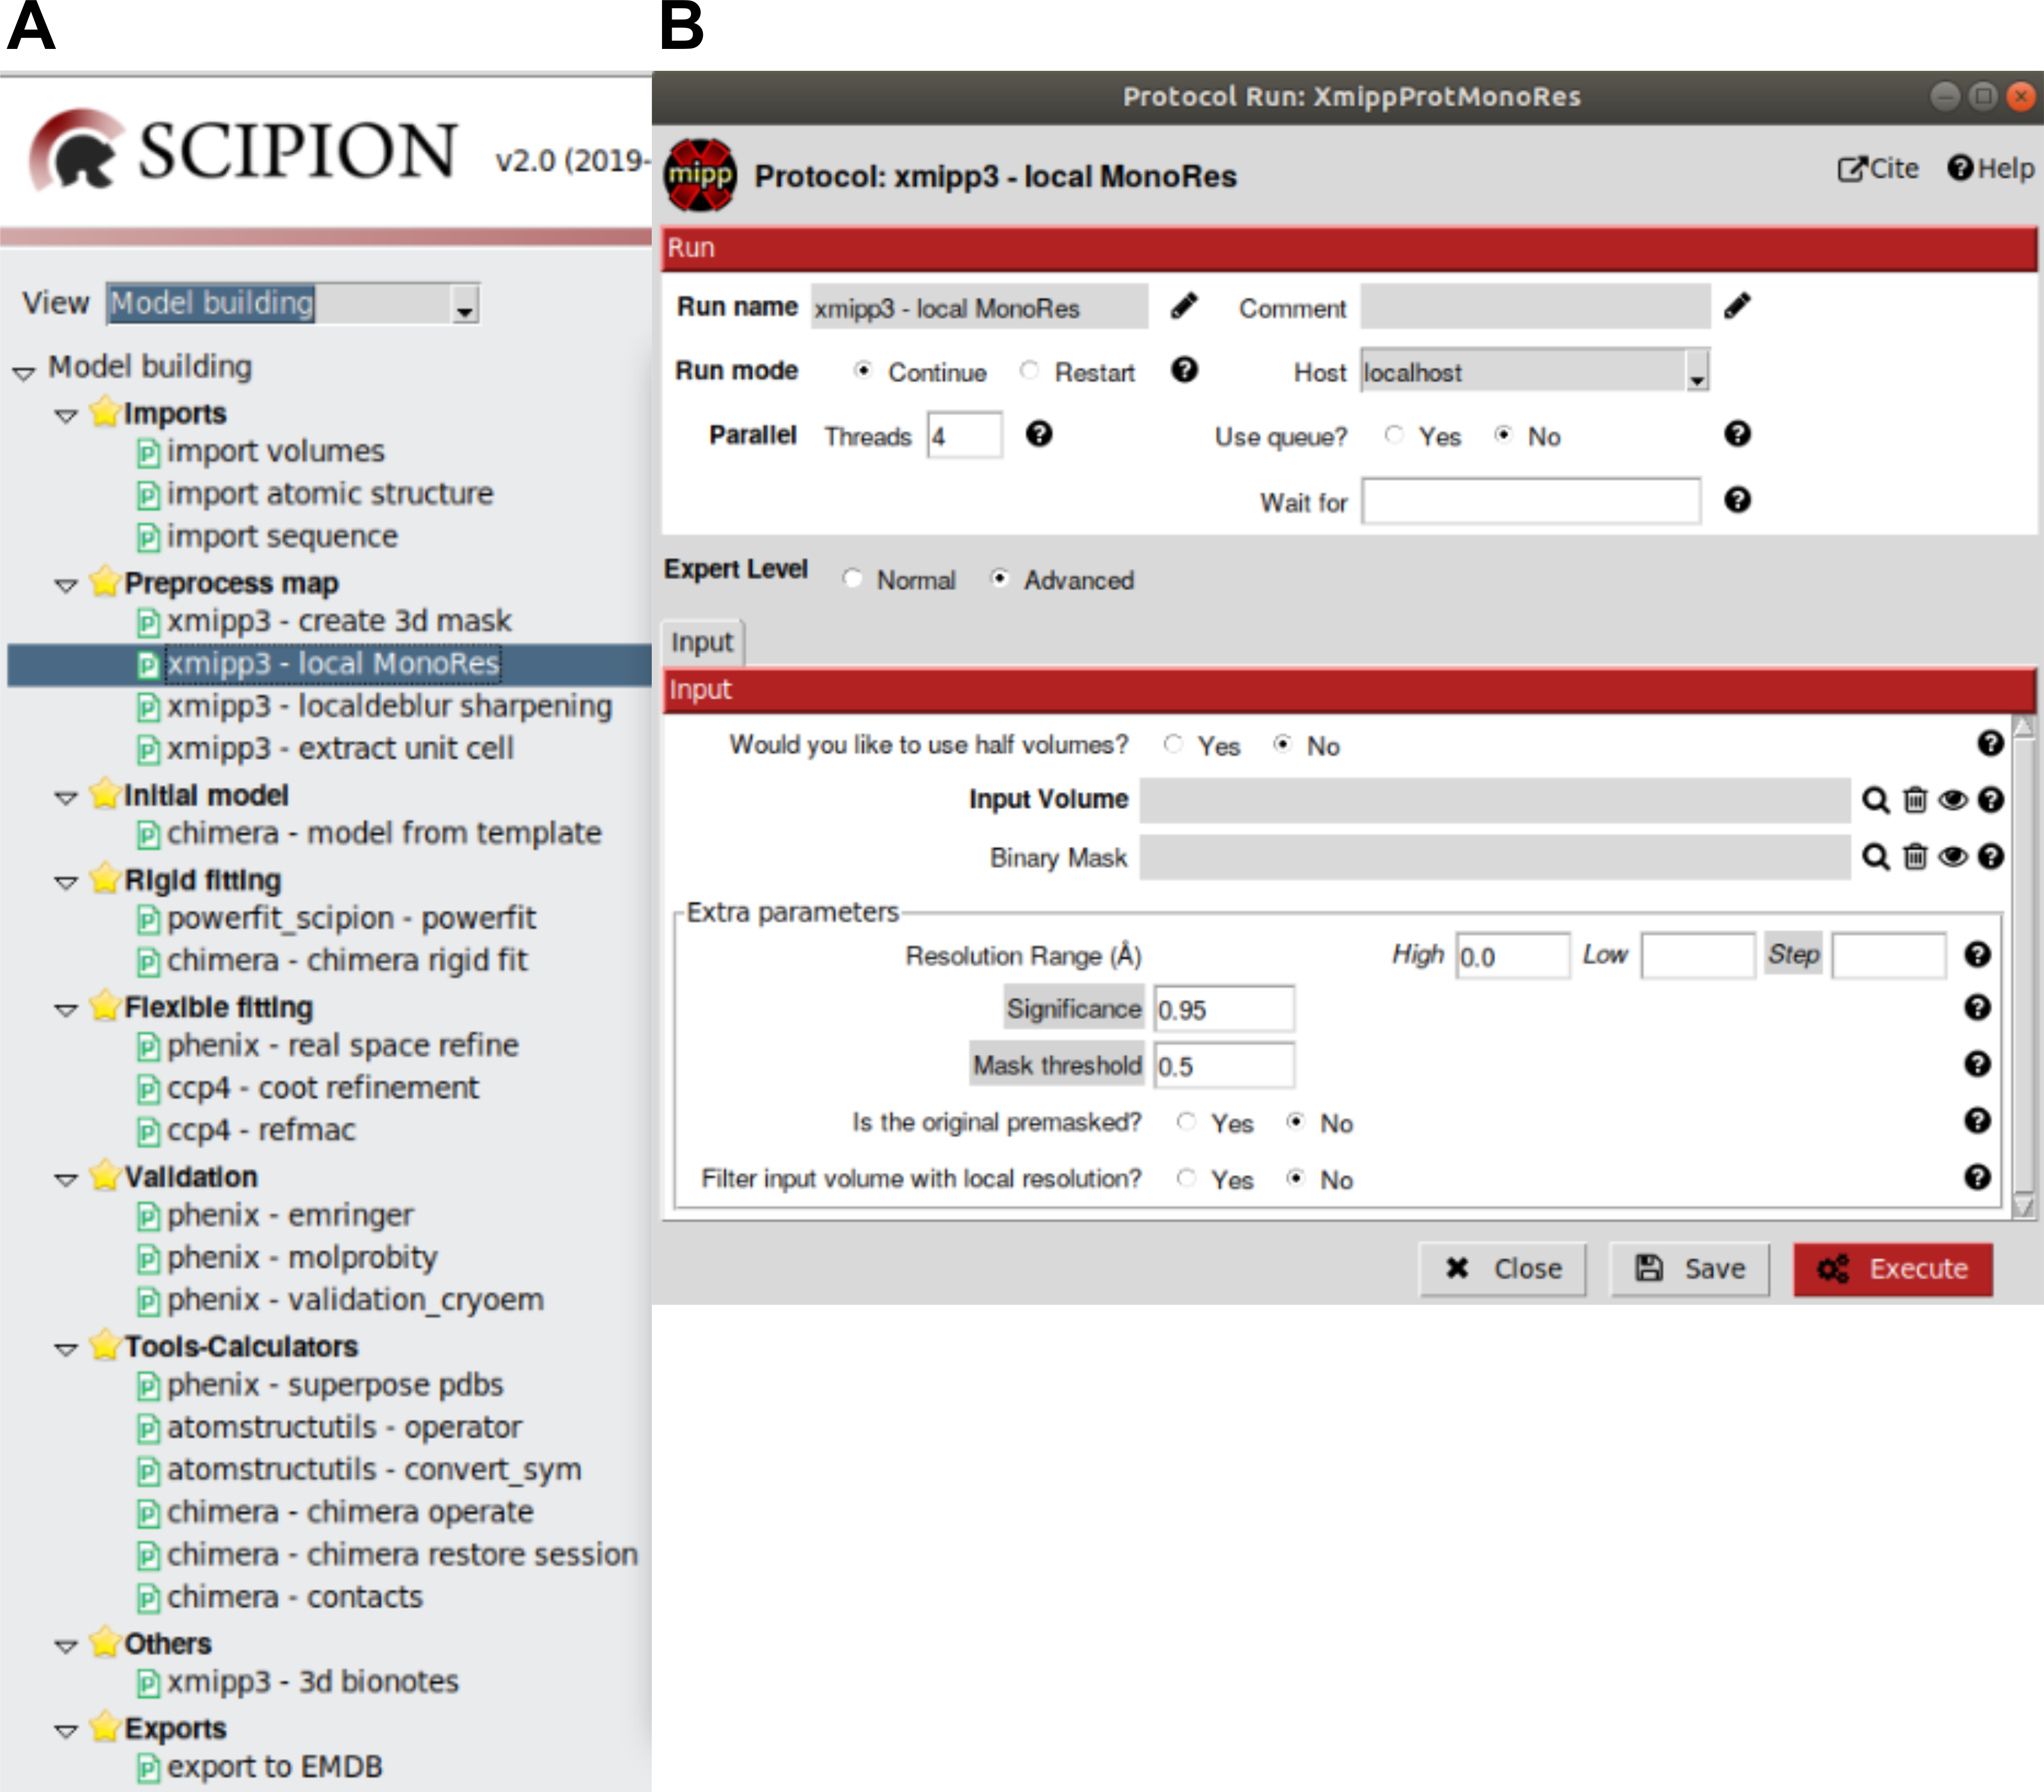
\includegraphics[width=0.90\textwidth]{Images_appendix/Fig207}
     \caption{Protocol \scommand{xmipp3 - local MonoRes}. A: Protocol location in \scipion menu. B: Protocol form.}
     \label{fig:app_localMonoRes_1}
    \end{figure}
    
    \begin{itemize}
        \item \ttt{Would you like to use half volumes?}: Option ``No'' has been selected by default, with the box \ttt{Input Volume} to fill in with the volume, imported or generated in \scipion. However, since the noise estimation needed to determine the local resolution is based on half volumes, select ``Yes'' when half volumes are available. A couple of boxes will thus be opened to select both half volumes, \ttt{Volume Half 1} and \ttt{Volume Half 2}.
        \item \ttt{Binary Mask}: Mask that will be overlapped to the map volume in order to indicate which points of the map are specimen and which are not.
         \item \ttt{Exclude area}: Advanced parameter to select part of the specimen that should be excluded from the estimation of local resolution, for example in viruses to exclude the inner genetic material or in membrane proteins to exclude fosfolipids. Remark that we are talking about part of the specimen (signal and not noise) in which we are simply not interested. 
        \item \ttt{Extra parameters}:
        \begin{itemize}
            \item \ttt{Resolution Range (\AA)}: Interval of resolution expected, from the maximum resolution (\ttt{High} = 0.0 by default), to the minimal resolution (\ttt{Low}) of the map volume. This parameter is empty by default and $MonoRes$ will try to estimate it. \ttt{Step} is an advanced parameter that indicates the fraction of resolution of each interval in the range contained between the max and min resolution. 
            \item \ttt{Significance}: Advanced parameter that determines the significance of the hypothesis test computed to calculate the resolution (0.95 by default).
            \item \ttt{Mask threshold}: Advanced parameter that indicates the density value required to get a binary mask in case there is not one (0.5 by default). Density values below the threshold will be changed to 0 and values above the threshold will be changed to 1.
            \item \ttt{Consider noise gaussian?}: ``No'' by default has to be changed to ``Yes'' if you prefer to establish the premise that the noise follows a gaussian distribution. 
        \end{itemize}
    \end{itemize}
  \item Protocol execution:\\
  Adding specific map/structure label is recommended in \ttt{Run name} section, at the form top. To add the label, open the protocol form, press the pencil symbol at the right side of \ttt{Run name} box, complete the label in the new opened window, press OK and, finally, close the protocol. This label will be shown in the output summary content (see below). If you want to run again this protocol, do not forget to set to \ttt{Restart} the \ttt{Run mode}.\\
  Press the \ttt{Execute} red button at the form bottom.
  
  \item Visualization of protocol results:
  
  After executing the protocol, press \ttt{Analyze Results} and a menu window will be opened (\ffigure{fig:app_localMonoRes_2}):
  
  \begin{figure}[H]
     \centering 
     \captionsetup{width=.7\linewidth} 
     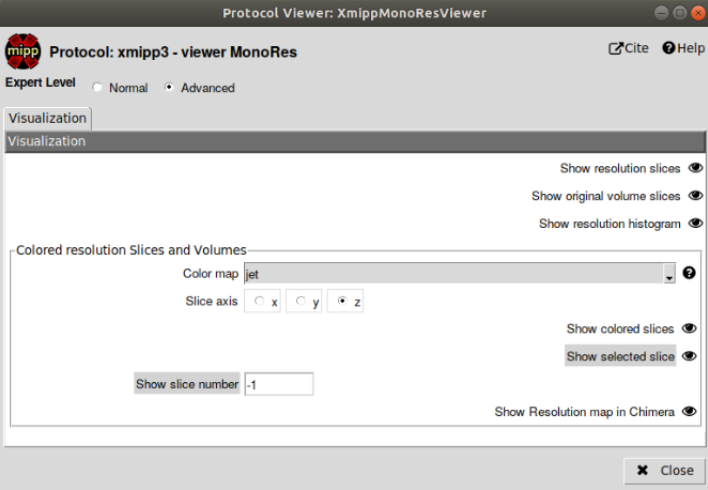
\includegraphics[width=0.70\textwidth]{Images_appendix/Fig209.pdf}
     \caption{Protocol \scommand{xmipp3 - local MonoRes}. Menu to visualize results.}
     \label{fig:app_localMonoRes_2}
    \end{figure}
    
   \begin{itemize}
     \item \ttt{Show resolution slices}: Map resolution slices are opened with $ShowJ$ (\url{https://github.com/I2PC/scipion/wiki/ShowJ}), the default \scipion viewer.
     \item \ttt{Show original volume slices}: Original map slices are opened with $ShowJ$.
     \item \ttt{Show resolution histogram}: Number of map voxels that show a certain resolution.
     \item \ttt{Colored resolution Slices and Volumes}: Box that allows to display local resolution of map and slices according to a specific color code.
     \begin{itemize}
        \item \ttt{Slice axis}: Select the perpendicular axis to visualize the slices. The \ttt{Z} axis is perpendicular to the screen.
        \item \ttt{Show colored slices}: Map slices 34, 45, 56 and 67 of local resolution along the axis selected previously.
        \item \ttt{Show selected slice}: Advanced parameter to show by default the 51 local resolution slide, or any other selected along the axis selected previously.
        \item \ttt{Show slice number}:  Advanced parameter to select the slice number to be shown by \ttt{Show selected slice}.
        \item \ttt{Show Resolution map in ChimeraX}: The resolution map is shown using $ChimeraX$. Left hand bar indicates resolution colour code.
        \item
        \begin{itemize}
            \item \ttt{Color scale options}: Highest value of the resolution range.
            \item \ttt{Lowest}: Lowest value of the resolution range.
            \item \ttt{Intervals}: Number of resolution intervals from the highest to the lowest range value.
            \item \ttt{Color set}: Color to apply to the local resolution map (\url{http://matplotlib.org/1.3.0/examples/color/colormaps_reference.html}).
        \end{itemize}  
        \ttt{Note}: Remark that on the right side you have a wizard to control color params.
     \end{itemize}
   \end{itemize} 


 \item Summary content:
  \begin{itemize}
     \item Protocol output (below \scipion framework):\\ \ttt{xmipp3 - local MonoRes -> resolution\_Volume};\\ Volume (x, y, and z dimensions, sampling rate).
     \item \ttt{SUMMARY} box:\\ \ttt{Highest resolution} and \ttt{Lowest resolution}.
    \end{itemize}
    
\end{itemize}
